\chapter{Multipartite Entanglement Stabilization}
%
The central goal of quantum optics is to develop ``tools" to control light-matter interactions at the single quanta level. Chiral interfaces, such as light scattering off an atom and the photoelectric effect, are interesting examples where photon emission and absorption is non-reciprocity arising from the polarization-dependent coupling strength. These phenomena are dealt within the framework of \textit{chiral quantum optics}. For our purposes we'll be interested `one-dimensional' interfaces where quantum emitters (atoms/qubits) interact with guided modes of light with in a waveguide. These system display unidirectional emission and absorption where an emitter can interact with another emitter, via a photon, only if it is further down the chain.  Theses systems naturally give rise to chiral couplings \cite{Chiral_Quantum_Optics,Chiral_QO_of_Spin_Chains}. 

Building upon ideas developed in the last chapter, we will consider a chain of a qubits coupled to mutual resonator that realizes pairwise chiral couplings between qubits to create effective unidirectional emission and absorption within the qubit system. We find that in the chiral system, the nature of entanglement can be modified from two-qubit to multi-qubit by selecting the suitable driving condition: specifically, the detunings of the driving fields from respective qubit frequencies. The nature of the entanglement generated in steady state will be investigated by looking at purity of qubit subspaces spanning 1, 2, 3 and 4 qubits respectively. We will also comment on how  multipartite entanglement can be realized without chirality, though at the cost of introducing additional constraints on the system.

%As was suggested in the last chapter, chiral stabilization seem to stabilize bell states ``better". In this chapter we'll show that chiral couplings can be used for the purification of four-way entangled states. To identify four-way entanglement we'll investigate the purity of the qubit sub spaces. 


\section{Four-qubit engineered dissipator}
\begin{figure} \label{Fig:Detuning Pattern}
    \centering
    
\subfigure[]{
     \begin{tikzpicture}[x=1.0in,y=1.0in]
    \draw[color=black!100 , ultra thick] (0,0) parabola (0.6,1.08) ;
    \draw[color=black!100 , ultra thick] (0.0,0.0) parabola (-0.6,1.08) ;
    \draw[color=black!100 , ultra thick] (-0.36514837167011072,.4) -- (0.36514837167011072,.4);
    \draw[color=black!100 , ultra thick] (0.2581988897471611,.2) -- (-0.2581988897471611,.2);
    \draw[color=black!100 , ultra thick] (0.44721359549995793,.6) -- (-0.44721359549995793,.6);
    \draw[color=black!100 , ultra thick] (0.5163977794943222,.8) -- (-0.5163977794943222,.8);
    \draw[color=black!100 , ultra thick] (0.57735026918962573,1.0) -- (-0.57735026918962573,1.0);
    \draw[color=black!100, ultra thick](-.75,-1) circle (.3);
    \node at (-.75 , -1.5){\scalebox{1.25}{$\delta_2$}} ;
    \draw[color=black!100, ultra thick](.75,-1) circle (.3);
    \node at (.75 , -1.5){\scalebox{1.25}{$\delta_{3}$}} ;
    %\draw[dotted , ultra thick] (.25,-1) -- (-.25,-1);
    \draw[color= black!100 , ultra thick] (-.6,-1.15)--(-0.9,-1.15);
    \draw[color= black!100 , ultra thick] (-.6,-.85)--(-0.9,-0.85);
    \draw[color= black!100 , ultra thick] (.6,-1.15)--(0.9,-1.15);
    \draw[color= black!100 , ultra thick] (.6,-.85)--(0.9,-0.85);
    \draw[color= black!100 , ultra thick] (-1.85,-1.15)--(-2.15,-1.15);
    \draw[color= black!100 , ultra thick] (-1.85,-.85)--(-2.15,-0.85);
    \draw[color= black!100 , ultra thick] (1.85,-1.15)--(2.15,-1.15);
    \draw[color= black!100 , ultra thick] (1.85,-.85)--(2.15,-0.85);
    \draw[color=black!100, ultra thick](-2,-1) circle (.3);
    \node at (-2.0 , -1.5){\scalebox{1.25}{$\delta_1$}} ;
    \draw[color=black!100, ultra thick](2,-1) circle (.3);
    \node at (2.0 , -1.5){\scalebox{1.25}{$\delta_{4}$}} ;
    \draw[black, ultra thick , tipA-tipA] (-0.6,-.65) -- (-0.3,0.1);
    \draw[black, ultra thick , tipA-tipA] (0.6,-.65) -- (0.3,0.1);
    \draw[black, ultra thick , tipA-tipA] (1.75,-.75) -- (0.35,0.2);
    \draw[black, ultra thick , tipA-tipA] (-1.75,-.75) -- (-0.35,0.2);
    \end{tikzpicture}
}

\subfigure[]{
\begin{tikzpicture}[x=1.0in,y=1.0in]
\draw[color=black!100, ultra thick](.5,.5) circle (.3);
\node at (-0.93 , 0.5){\scalebox{1.25}{$\delta_1$}} ;
\draw[color=black!100, ultra thick](.5,-.5) circle (.3);
\node at (0.93 , 0.5){\scalebox{1.25}{$\delta_2$}} ;
\draw[color=black!100, ultra thick](-.5,.5) circle (.3);
\node at (-0.93 , -0.5){\scalebox{1.25}{$\delta_4$}} ;
\draw[color=black!100, ultra thick](-.5,-.5) circle (.3);
\node at (0.93 , -0.5){\scalebox{1.25}{$\delta_2$}} ;
\draw[dashed , ultra thick , tipA-tipA] (.2,.5) -- (-.2,.5);
\draw[dashed , ultra thick , tipA-tipA] (.2,-.5) -- (-.2,-.5);
\draw[dashed , ultra thick , tipA-tipA] (.5,.2) -- (.5,-.2);
\draw[dashed , ultra thick , tipA-tipA] (-.5,.2) -- (-.5,-.2);
\draw[color= black!100 , ultra thick] (.65,.35)--(.35,.35);
\draw[color= black!100 , ultra thick] (.65,.65)--(.35,.65);
\draw[color= black!100 , ultra thick] (-.65,.35)--(-.35,.35);
\draw[color= black!100 , ultra thick] (-.65,.65)--(-.35,.65);
\draw[color= black!100 , ultra thick] (.65,-.35)--(.35,-.35);
\draw[color= black!100 , ultra thick] (.65,-.65)--(.35,-.65);
\draw[color= black!100 , ultra thick] (-.65,-.35)--(-.35,-.35);
\draw[color= black!100 , ultra thick] (-.65,-.65)--(-.35,-.65);
\draw[dashed , ultra thick , tipA-tipA] (-.2878679656440358,-.2878679656440358)--(.2878679656440358,.2878679656440358);
\draw[dashed , ultra thick , tipA-tipA] (.2878679656440358,-.2878679656440358)--(-.2878679656440358,.2878679656440358);
\node at (0, 1.0){\underline{\scalebox{1.25}{Symmetric}}} ;
\end{tikzpicture}
}\hspace{3cm}
\subfigure[]{
\begin{tikzpicture}[x=1.0in,y=1.0in]
\draw[color=black!100, ultra thick](.5,.5) circle (.3);
\node at (-0.93 , 0.5){\scalebox{1.25}{$\delta_1$}} ;
\draw[color=black!100, ultra thick](.5,-.5) circle (.3);
\node at (0.93 , 0.5){\scalebox{1.25}{$\delta_2$}} ;
\draw[color=black!100, ultra thick](-.5,.5) circle (.3);
\node at (-0.93 , -0.5){\scalebox{1.25}{$\delta_4$}} ;
\draw[color=black!100, ultra thick](-.5,-.5) circle (.3);
\node at (0.93 , -0.5){\scalebox{1.25}{$\delta_3$}} ;
\draw[ ultra thick , tipA-] (.2,.5) -- (-.2,.5);
\draw[ ultra thick , -tipA] (.2,-.5) -- (-.2,-.5);
\draw[ ultra thick , -tipA] (.5,.2) -- (.5,-.2);
\draw[ ultra thick , -tipA] (-.5,.2) -- (-.5,-.2);
\draw[color= black!100 , ultra thick] (.65,.35)--(.35,.35);
\draw[color= black!100 , ultra thick] (.65,.65)--(.35,.65);
\draw[color= black!100 , ultra thick] (-.65,.35)--(-.35,.35);
\draw[color= black!100 , ultra thick] (-.65,.65)--(-.35,.65);
\draw[color= black!100 , ultra thick] (.65,-.35)--(.35,-.35);
\draw[color= black!100 , ultra thick] (.65,-.65)--(.35,-.65);
\draw[color= black!100 , ultra thick] (-.65,-.35)--(-.35,-.35);
\draw[color= black!100 , ultra thick] (-.65,-.65)--(-.35,-.65);
\draw[ ultra thick , tipA-] (-.2878679656440358,-.2878679656440358)--(.2878679656440358,.2878679656440358);
\draw[ ultra thick , tipA-] (.2878679656440358,-.2878679656440358)--(-.2878679656440358,.2878679656440358);
\node at (0, 1.0){\underline{\scalebox{1.25}{Chiral}}} ;
\end{tikzpicture}
}
\caption{Four qubits coupled to a mutually shared resonator mode, with an associated detuning pattern $( \delta_1 , \delta_2 , \delta_3 , \delta_4)$. (b) In the symmetric scheme all qubits are coupled to each other through a dissipative coupling. (c) Addition of qubit-qubit couplings, and their interference with the dissipative couplings, renders all pairwise couplings in the chain unidirectional, such that the qubits on the left cannot ``see" the qubits to their right.}
\end{figure}
%
Consider a chain of four qubits interacting with a mutual resonator, as depicted in  system Fig. \ref{Fig:Detuning Pattern}(a). We assume homogeneous couplings, $g_i=g$, so
%
\begin{equation}
    \frac{H_{SR}'}{\hbar} = g b^\dagger ( \sigma_1 + \sigma_2 + \sigma_3 + \sigma_4) + h.c.
\end{equation}
%
Using the adiabatic elimination of the resonator, as described in the previous chapter, this allows a straightforward identification of the effective junp operator
%
\begin{eqnarray}
    \hat{S} = g ( \sigma_1 + \sigma_2 + \sigma_3 + \sigma_4)
\end{eqnarray}
%
which leads to the following master equation for the reduced system
%
\begin{equation}\label{four qubit}
    \dot{\rho}_S = - \frac{i}{\hbar} [H_S' , \rho_S] + \Gamma \mathcal{L}[\sigma_1 + \sigma_2 + \sigma_3 + \sigma_4] \rho_S.
\end{equation}
%
As before, $\Gamma = \frac{4g^2}{\kappa}$ is the engineered dissipation rate. Associated with each of the qubits is a detuning, $\delta_\alpha$, also depicted in in Fig. \ref{Fig:Detuning Pattern}(a). These detunings must come in equal and opposite pairs to form a perfectly coherent emitter-absorber with no spontaneous emission into the guided mode \cite{Cascade_Quantum_Systems}. That is for each qubit $j$ with a detuning $\delta_j$, there is another qubit $l$ in the chain with $\delta_j = - \delta_l$. 
%
\par
%
We will again consider the stabilization dynamics for both:
%
\begin{itemize}
\item a symmetric interaction between each pair of qubits, for which the qubit Hamiltonian is invariant under pairwise permutations [Fig. \ref{Fig:Detuning Pattern}(b)],
\begin{equation}
    H_{sym} = \sum_i \left( \frac{\delta_i}{2} \sigma_{zi} + \frac{\Omega}{2} \sigma_{xi} \right)
\end{equation}
\item a chiral interaction between each pair of qubits, for which the qubit Hamiltonian is no longer invariant under pairwise permutations [Fig. \ref{Fig:Detuning Pattern}(c)],
\begin{equation}
   H_{chiral} = H_{sym} - i \frac{\Gamma}{2} \sum_{i > j} \left( \sigma_j^\dagger \sigma_i - \sigma_j \sigma_i^\dagger \right)
\end{equation}
This is because the qubit-qubit couplings pick up a phase under an index swap. Recall that the combination of these couplings with engineered dissipation creates unidirectional emission and absorption from left-to-right in the chain, as demonstrated for the Bell state stabilization in the last chapter.
\end{itemize}
%
%
%We will find that the detuning pattern will determine whether four-way entanglement arises in the qubits space. First we will show how the purity of qubit subspace can be used to determine entanglement. Finally we will consider entanglement in the symmetric and chiral stabilization scheme. 
%
%The asymmetric part is responsible qubit-qubit couplings so that the net driven-dissipative interaction is chiral. Each of the qubits is driven symmetrically that is $\Omega_i = \Omega$. Furthermore the detunings between qubit pairs that chancel out so that for every qubit qubit $i$ in the chain with a detuning $\delta_i$ there is another qubit $l$ in the chain with a detuning that satisfies $\delta_i = - \delta_l$. When these conditions are satisfied the qubit chain will dimeraterize. That is the steady state of the qubit chain can be in terms of different dimers
%
\section{Role of chirality}
%
We consider the entanglement dynamics in the symmetric and chiral case for two different types of detuning patterns: alternating and staggered. An alternating detuning pattern is of the form $(\delta_a , - \delta_a , \delta_b , - \delta_b )$. A staggered detuning is obtained by permuting two of the detunings: $(\delta_a , \delta_b , -\delta_a , - \delta_b )$.
%
\par
%
\subsection{Entanglement Identification}
%
In order to identify the nature of multipartite entanglement in each case, we use a quantity called the purity of the density matrix: $tr
\left( \rho^2 \right)$. The purity of the density matrix has the following property
 \begin{eqnarray}
 tr( \rho^2 ) & = & 1 \quad\text{ for a pure state} \nonumber \\
  tr( \rho^2 ) & < & 1 \quad\text{ for a mixed state}. \nonumber
 \end{eqnarray}
Now suppose two subsystem in the chain are entangled. Then by definition the total state, $| \Phi \rangle$, cannot written as a product state of the two subsystems. That is 
 \begin{equation}
 |\Phi \rangle \neq |\phi_1 \rangle \otimes |\phi_2 \rangle.
 \end{equation}
 Therefore when one of the subsystems is traced over, the resulting density matrix is mixed with a purity less than one \cite{Entangle_Time_Scale}. For example, suppose two qubits $j$ and $k$ in the chain are entangled.
\begin{equation}
| S \rangle_{j k } = \frac{1}{\sqrt{2}} \left( | g e \rangle_{j k } - | e g \rangle_{ j k } \right)
\end{equation}
We trace over the subspace $j$ and find
\begin{equation}
    \rho_{k} = tr_j \lbrace | S \rangle_{j k }\langle S | \rbrace = \frac{1}{2} \left(| e \rangle_k \langle e | + | g \rangle_k \langle g |\right) = \frac{1}{2} \left( \begin{array}{cc}
       1  & 0 \\
       0  & 1
    \end{array} \right).
\end{equation}
Computing $tr_k \left\lbrace \rho_k^2 \right\rbrace = 0.5 < 1 $, we see that the subsystem is mixed and its purity is less than one.
%
\subsection{Alternating Detunings}
%
The results for purity plots are shown in Fig. \ref{fig:alternating}. Our results show that both the symmetric and chiral schemes purify the state $|S\rangle_{12} | S \rangle_{34}$. However, the chiral purification is faster by more than a factor of 10. Furthermore, in the chiral case $|S\rangle_{12}$ is stabilized before $|S\rangle_{34}$ displaying the system's unidirectional nature.
%
\begin{figure}[t!]
%    \textbf{$\Gamma= 4\frac{g^2}{\kappa}=10 \; \delta_a = 1 \; \delta_b = 4 , \Omega=8$}\par
%    \textbf{$(\delta_a , - \delta_a , \delta_b , - \delta_b )$}\par
\centering
\subfigure[]{
  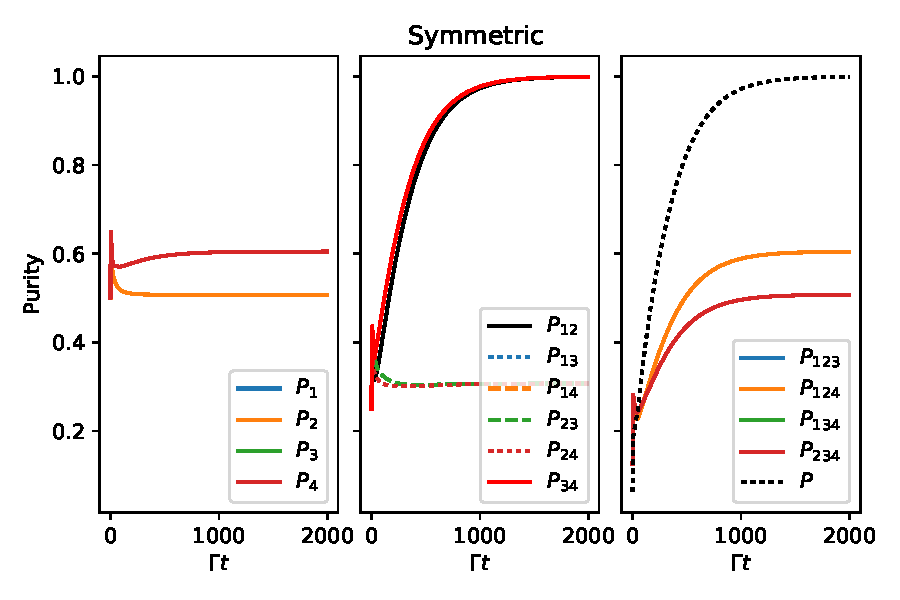
\includegraphics[scale=.85]{Images/Sym_Alternating.pdf}
}
\vspace{-.5cm}
\subfigure[]{
  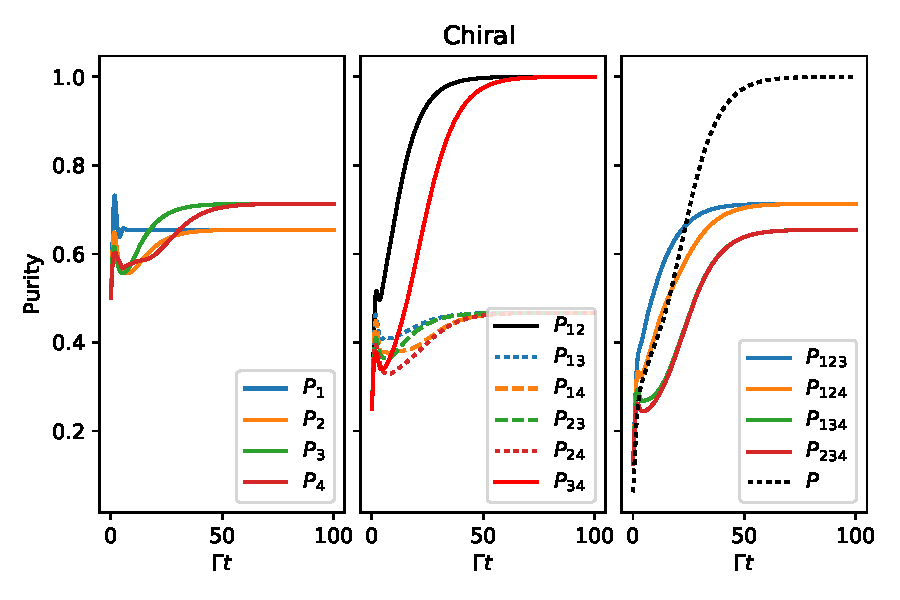
\includegraphics[scale=.85]{Images/Chiral_Alternating.pdf}
}
%\vspace{3mm}
    \caption{Time-domain simulations of a four-qubit chain for symmetric and chiral cases with alternating detuning pattern: $(\delta_a , - \delta_a , \delta_b , - \delta_b )$. All the plots were generated with the same parameters, $\Gamma= 4\frac{g^2}{\kappa}=10, \; \delta_a = 1, \; \delta_b = 4, \; \Omega=8$.}
    \label{fig:alternating}
\end{figure}
%
%
\subsection{Staggered Detunings}
%
The results for purity plots are shown in Fig. \ref{fig:staggered}. For the symmetric coupling case we get non-local (though still pairwise) entanglement, and the state $|S\rangle_{13}|S\rangle_{24}$ is purified. However, for chiral couplings, only the full 4-qubit system purity goes to one indicating that the steady state exhibits genuine four-qubit entanglement. 
%
\begin{figure}[h!]
%\textbf{$\Gamma= 4\frac{g^2}{\kappa}=10 \; \delta_a = 1 \; \delta_b = 4 , \Omega=8$}\par
%    \textbf{$(\delta_a , - \delta_a , \delta_b , - \delta_b )$}\par
\centering
\subfigure[]{
  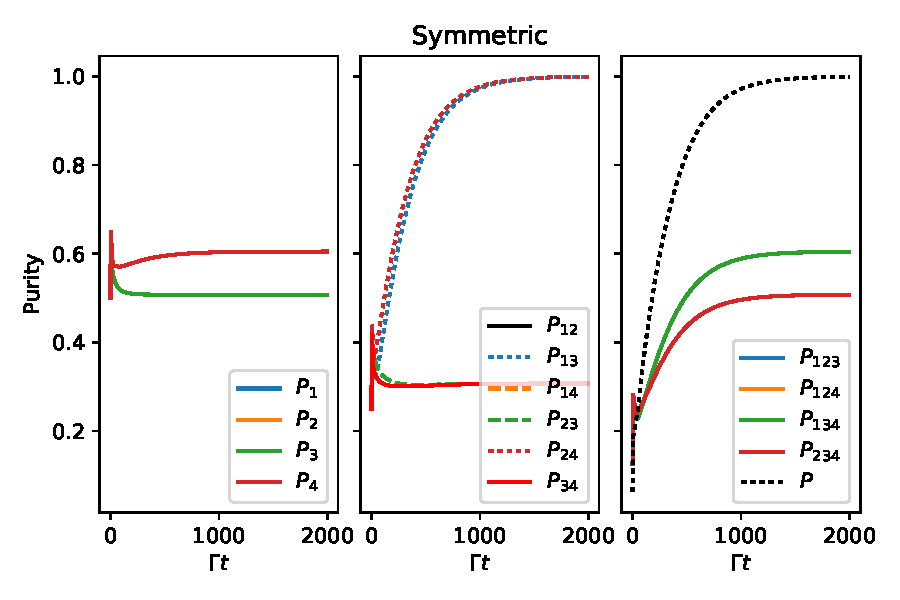
\includegraphics[scale=.85]{Images/Sym_Staggered.pdf}
}
\vspace{-.5cm}
\subfigure[]{
  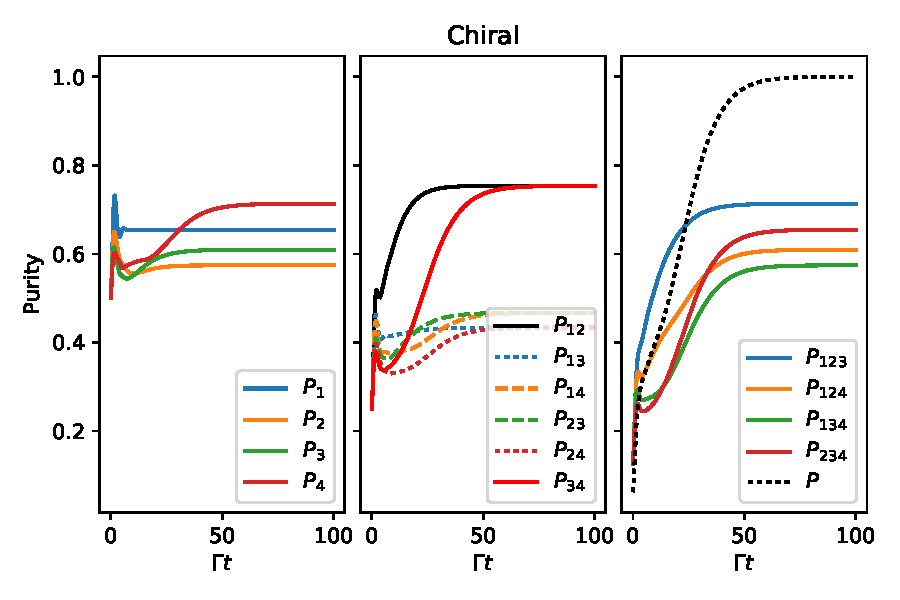
\includegraphics[scale=.85]{Images/Chiral_Staggered.pdf}
}
%\vspace{3mm}
    \caption{Time-domain simulations of a four-qubit chain for symmetric and chiral cases with staggered detuning pattern, $(\delta_a , \delta_b , - \delta_a , - \delta_b )$. All the plots were generated with the same parameters, $\Gamma= 4\frac{g^2}{\kappa}=10, \; \delta_a = 1, \; \delta_b = 4, \; \Omega=8$.}
    \label{fig:staggered}
\end{figure}
%
\section{Caveat: Symmetric Four-qubit Entanglement}
%
Consider the homogeneous detuning detuning pattern
\begin{equation}\label{Detuning_Pattern}
 ( \delta ,  \delta , -\delta , - \delta  ).
\end{equation}
The third and fourth qubit can both form a coherent emitter-absorber pair with the first qubit because the detunings are equal and opposite. In other words, the first qubit can become entangled with the third qubit or the forth qubit. Because there can be no preferred entangled state, we found that the steady state was a superposition of the two possible configurations. Thus the detuning pattern, Eq. (\ref{Detuning_Pattern}), stabilizes
\begin{equation}
 \frac{1}{\sqrt{2}}\left( | S \rangle_{13} | S \rangle_{24} + | S \rangle_{14} | S \rangle_{23} \right).
\end{equation}
However, for this scheme to work the system has to be initialized in the ground state,  i.e.
\begin{equation}
    \rho_S(0) = | gggg \rangle \langle gggg |.
\end{equation}
We found a significant decrease in steady state fidelity when intialized in a mixed state. Table 4.1 summarizes the different permutations of the detuning pattern and the corresponding four-qubit entangled states that get stabilized as a result.
%
\begin{table}[t!]\label{Bell State Table}
\centering
\begin{tabular}{c|c}
\centering
Detuning Pattern & Stabilized State \\
\hline
$( \delta , - \delta , \delta , - \delta  )$ & $| S \rangle_{12} | S \rangle_{34} - | S \rangle_{14} | S \rangle_{23}$  \\
$( \delta , - \delta , -\delta ,  \delta  )$ & $ | S \rangle_{12} | S \rangle_{34} + | S \rangle_{13} | S \rangle_{24}$  \\
$( \delta , \delta , - \delta , - \delta  )$  & $ | S \rangle_{13} | S \rangle_{24} + | S \rangle_{14} | S \rangle_{23}$ 
\end{tabular}
\caption{Table of detuning patterns and corresponding stabilized four-qubit entangled state).}
\end{table}
%
\begin{figure}[h!]
\centering
%    \textbf{$\Gamma= 4\frac{g^2}{\kappa}=10 \; \delta = 1 \; \Omega=8$}\par
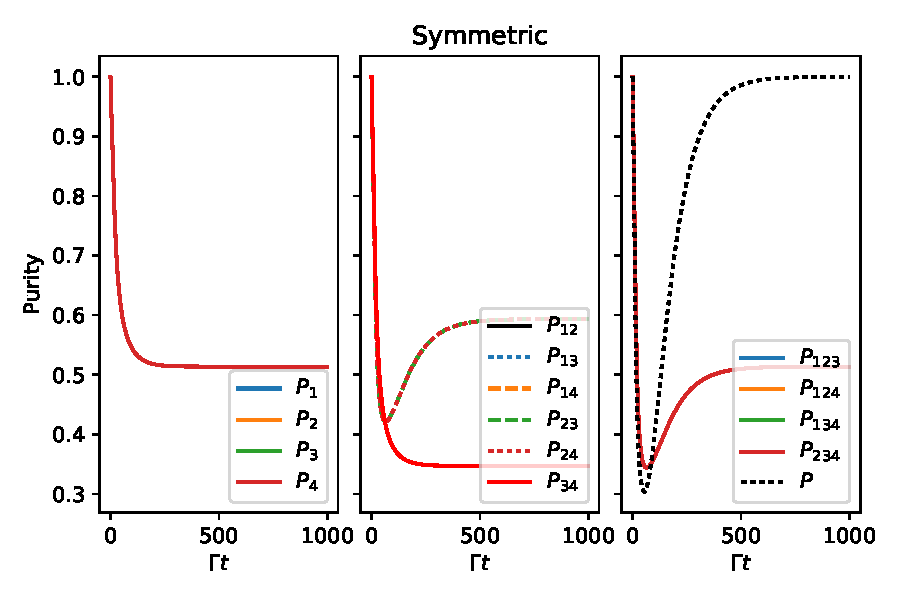
\includegraphics[scale=.85]{Images/Sym_Homo.pdf}
    \caption{Purity plots show that the steady state is a four-qubit entangled state when the system is initialized in the ground state, and the detuning pattern is homogeneous. The parameters used for the simulation were $\Gamma= 4\frac{g^2}{\kappa}=10, \; \delta = 1, \; \Omega=8$.}
    \label{fig:}
\end{figure}